\documentclass[conference]{IEEEtran}

\usepackage{algorithm}
\usepackage{algorithmic}
\usepackage{amsmath,scalerel}
\usepackage{graphicx}

\hyphenation{op-tical net-works semi-conduc-tor IEEEtran}
\begin{document}


\title{\LARGE Predicting Dubai Housing Prices with Machine Learning and Deep Learning Models}

\author{By Fardin Ahsan, Omar Al Shared, Khalifa Bin Thani and Chibuike Okika. }



\maketitle

\begin{abstract}
Housing prices in Dubai are not easily predictable for someone on the ground. This is because of the inherent quirks of Dubai's urban planning; one of which is multi-lane highways that run through the city centres. However, using Machine Learning, features that influence pricing can be determined and a predictive model can be built which can be used by potential buyers and sellers to estimate the market price of a house. This paper uses a tuned XtremeGradientBoost (XGB) model and a custom built Deep Neural Network (DNN) to tackle the task of predicting housing prices in Dubai. 
\end{abstract}
\IEEEoverridecommandlockouts
\begin{keywords}
Dubai housing prices, XtremeGradientBoost (XGB), Deep Neural Network (DNN).
\end{keywords}
% no keywords

% For peer review papers, you can put extra information on the cover
% page as needed:
% \begin{center} \bfseries EDICS Category: 3-BBND \end{center}
%
% for peerreview papers, inserts a page break and creates the second title.
% Will be ignored for other modes.
\IEEEpeerreviewmaketitle




\end{enumerate}


\section{Introduction}
Dubai has become a household name in real estate over the last few years and there are many types of real estate in the market. Obviously with the advancements in real estate, the valuation of property has been inflating as of late [1]. Prices of properties will differ, and the attributes and features of the housing property will always be reason behind these differences. The price will always be decided by factors such as the location and size of the property.
Location makes a huge difference in regards to the house prices. A house near or within the Dubai Centrepoint will obviously cost more than a house near the outskirts of Dubai. Additionally, A house that is on the beach will also cost more than a house that isn’t. All these factors come into play in regards to location and its effects on house prices.
The size of the property itself massively affects the house prices as well. Houses with more bedrooms and facilities will be valued much more than others. These structural characteristics will offer much more luxury to the potential buyers, therefore increasing the house’s value [2].
However, it is worth mentioning that having access to shopping malls or metro stations can be categorized in an attribute called neighbourhood. Community social status and the proximity of these facilities typically improve the property’s worth [2].
Methods on preparing the data include data cleaning. Training sets can be refined by data cleaning techniques to get rid of uncorrelated information related to the prices. In some cases, the training sets wouldn’t require as much refinement. After that is done, the attributes can be utilised by Machine learning (ML) models to predict the house prices.

\section{Background}
Xtreme Gradient Boosting (XGBoost) is an implementation of gradient boosted decision trees designed for speed, performance and optimization. XGBoost concepts builds on supervised machine learning, decision tree, ensemble and gradient boosting. It is a combination of software and hardware optimization techniques in order to get excellent results using less computing resources in less time. XGBoost can be used to solve regression and classification problems. We will be using it predicting house prices in Dubai. Dealing with prediction problems that has to do with unstructured data such as images and text, artificial neural networks will tend to outperform all other algorithms. Nonetheless, for small-to-medium structured or tabular data, and especially data with a majority of Boolean features, XGBoost tends to stand out, hence our usage for this project.
Some of the good features of XGBoost algorithm is that it runs smoothly on Windows, Linux, and OS X and supports all major programming languages like Python, C++, Java, Scala, and Julia. It also has good cloud integration. XGBoost is more regularized form of Gradient Boosting. XGBoost uses advanced regularization (L1 & L2), which improves model generalization capabilities. XGBoost delivers high performance as compared to Gradient Boosting. Its training is very fast and can be parallelized / distributed across clusters [3]. XGBoost is a scalable tree boosting system.
We also made use of Deep Neural Network in this work. A neural network or sometimes called Artificial Neural Network (ANN) is simply a series of algorithms that endeavors to recognize underlying relationships in a set of data through a process that mimics the way the human brain operates [4]. It can adapt to changing input of which would make the network to generate the best possible result without needing to redesign the output criteria.
Deep Neural Network (DNN), is a neural network with a certain level of complexity, a neural network with more than two layers. It uses multivariate mathematical modeling to process complex. Deep neural networks have recently become the standard tool for solving a variety of computer vision problems and prediction problems.




\section{Literature Review}
There is a great deal of literature on the subject of using machine learning models to predict housing and property prices. Ahtesham et al state in their study that using an XGBoost algorithm has yielded the best and most accurate result with a model accuracy of 98%. The author also suggests that XGboost is faster than some alternatives for their dataset as it is a suitable algorithm for tabular datasets and is capable of parallel processing making it up to 10 times faster than alternative models [3].       
	In a study conducted by Kumar et al, a system that automatically predicts the price of a house the most accurately was designed. Multiple regression algorithms were compared and the performance of each model was assessed Root Mean Square Error (RMSE). This metric was chosen as it punishes outliers greatly and would thus help differentiate between the performance of each model. They tested many models and found that Catboost regression yielded the lowest RMSE. Catboost regressor is an algorithm well suited for text, image, and historical, as well as requiring less training than other similar models. It was well suited for this study as the dataset was of historical sales data [4].   
	Some studies sought to use neural networks in conjunction with regression algorithms. One such study conducted by Varma et al utilized linear regression, forest regression, and boosted regression initially. The results were then fed into a neural network that was applied with boosted regression to increase the accuracy of the model. The neural network improves the results by computing the results fed into it from the previous regression models and computes the best result out of them. The study concludes that a combination of multiple regression models achieves better results than a single model. [5]   
	Work done by Truong et al looked at using multiple machine learning models to identify the differences amongst them. 5 models were tested: Random forest, XGBoost, LightBGM, Hybrid regression, and Stacked Generalization. Hybrid regression and stacked generalization utilize more than one regression algorithm in their model. Hybrid regression is a combination of, in the case of this study, 3 algorithms; Random Forest, XGBoost, and LightGBM. Stacked generalization consists of a 2-level stacking architecture where the first level consists of a regression algorithm whose results are fed into the next level as features for another regression algorithm. The results of the study found that Random Forest showed the best results but is prone to overfitting, while XGBoost and LightGBM weren’t prone to overfitting but not as accurate. While these 3 models required tuning and optimization to produce satisfactory results, Hybrid regression and stacked generalization did not require any tuning or optimization. Interestingly stacked generalization did poorly on the training set but performed well on the test set. This is likely due to the use of 5-fold cross-validation and a coupling effect with the regression models in use where they supported each other to produce better results. The only problem with it is that the time complexity is quite high. Overall the tested models all yielded satisfactory results with some advantages over the others, the best model would depend on the dataset being used. [6]        
There was research carried out to evaluate the use of deep learning alongside XGBoost regression in estimating the price of real estate. Zhao et al sought to incorporate images of property in conjunction with tabular data to increase the accuracy of predictions. A hybrid neural network was built consisting of 4 components: A convolutional neural network was trained on AVA to give scores to property images. A multilayer perceptron model to analyze data from a table. One more CNN to extract specific visual features from the images. And finally, XGBoost regression to predict the final price of the property. The study found that a hybrid neural network improved the accuracy of the predictions by utilizing features that are typically not considered, such as images showing the aesthetic or quality of a house. [7]      
Identifying the major factors that affect the price of a house can help in identifying major features. In [8], the Spearman correlation coefficient was used to identify the major factors that affect the price: Environmental factors (the surroundings of the house), House factors (the specifications of the house itself), and transportation factors. These factors were then used in a multiple linear regression to predict the prices of houses. The study shows that identifying key features can improve the performance of a regression model. [8]
	In a study seeking to predict real estate prices in Finland, [9] sought to improve the existing artificial neural networks’ performance by automatically optimizing their hyperparameters. A baseline ANN model was used to compare against the optimized models. The fine-tuning of the hyperparameters was done automatically using a Bayesian algorithm, using the mean square error as the metric to measure the improvement. Utilizing Bayesian optimization improved the model in all metrics measured and did not show any over or underfitting. The paper concludes that using automatic tuning for the hyperparameters of a neural network is an effective way to improve the accuracy of results, and perhaps expanding the optimization process may yield even better results.  
The Journal of Property Study featured a paper on using machine learning algorithms to predict property prices. 3 regression models were trained and tested on a dataset of 40,000 housing transactions over 18 years in Hong Kong. The 3 models tested were: Support vector machine (SVM), Random Forest (RF), and Gradient Boost Machine (GBM). The results of the study concluded that RF and GBM performed the best in terms of accuracy. SVM, while not as accurate, was faster than both models. [10]   



%%%%
\section{Data set}

A total of 5 data sets were used to create the main data set that the models were trained on. 
'dubai\_sales' was the main training set. As shown in TABLE 1, it included apartment sales data from Dubai of 1844 unique apartments, along with the apartments features (it's area in square foot, does it have a swimming pool or not?, etc.), it's location and the neighborhood it belong to, and finally the price it was sold at. The price is the target of our modelling. 

\smallbreak
\smallbreak
\smallbreak
\scriptsize
\begin{tabular}{|l|l|l|l|l|}

\hline
\textit{\textbf{Dataset}} & \textit{\textbf{Role}} & \textit{\textbf{Description}} & \textit{\textbf{Size}} & \textit{\textbf{File format}} \\ \hline
dubai\_sales     & Training set            & Apartment sales data & 1844x36  & csv     \\ \hline
dubai.geojson    & Feature addition & Geospatial data      & - & geojson \\ \hline
dubai\_pop\_2019 & Feature addition & Demographic data     &  227x4 & csv     \\ \hline
dubai\_venues    & Feature addition & Venues data          &  2956x20 & csv     \\ \hline
dubai\_metros    & Feature addition & Metro stations data  &  561x7 & csv     \\ \hline

\end{tabular}
\smallbreak
\centrecaption{TABLE 1. Data sets used}
\smallbreak
\normalsize
The other data sets were used to augment features into the main data set, The 'neighborhood' column was used as the primary key to merge all the data sets to the primary training set. Firstly 'dubai.geojson' was used to gather geospatial data about Dubai, mainly the neighborhoods geographic outlines, this allowed for us to map the metro stations to the neighborhood they belonged to using their GPS coordinates, as 'dubai\_metros' didn't contain a neighborhood column. 

Finally 4 columns were added to the training set from the supplementary data sets, leading to a final size of 1844 rows and 40 columns.

\textit{Note: The data sets were collected from Kaggle.} [1]

%%%%%%%%%%
\section{Data preparation and Feature Engineering}
\subsection{Data cleaning}

As far as cleaning up the data set, there was little in the way. Mainly because the main training set did not have any null values, all 1844 rows and 76 columns had values. Thus the training set didn't require any pruning.

Three of the supplementary data sets (except for the data set on metro stations) had the same name for the neighborhoods. However, the names were not the same names as those in the primary set. In order to merge (similarly to a left merge in SQL) the supplementary set to the primary set, a dictionary was created manually mapping the names of the neighborhoods the primary set and the other sets had in common. Then it was a matter of replacing names using the mapping dictionary and merging the desired columns from the supplementary set to the primary set.

The data set for the metro stations did not have any neighborhood column. But it did contain the GPS coordinates for the metro stations, given we wanted to find out the number of metro stations in a neighborhood to add as a feature to the primary set, an algorithm was written to verify if a set of GPS coordinates fall within a neighbourhoods boundary polygon (present in 'dubai.geojson') and if yes, the metro station gets assigned that neighborhood. This allowed to merge the number of metro stations as a feature to the primary set. The algorithm is as follows as shown in Algorithm 1.


\begin{algorithm}
\caption{Map GPS coordinates to Neighborhood}
\begin{algorithmic} 
\FOR {$station$ in $station set$} 
\FOR {$neighborhood$ in $POLYGON$} 
\IF {$station(x,y)$ in $neighborhood$}
\STATE {assign neighborhood to station}
\ENDIF
\ENDFOR
\ENDFOR
\end{algorithmic}
\end{algorithm}



\subsection{Feature Engineering}

Once the desired features were extracted from the supplementary data sets as discussed in the 'Data Cleaning' section and merged into the main data set, the features had to be scaled such that they would work effectively and more importantly in a way that doesn't hinder the models' performance. 

\smallbreak
\smallbreak
\smallbreak
\smallbreak
\footnotesize
\begin{tabular}{|l|l|l|}
\hline
\textit{\textbf{Inherent   type}} & \textit{\textbf{Data type}} & \textit{\textbf{Process}} \\ \hline
GPS   coordinates            & float  & Convert to radians \\ \hline
Numerical   data             & float  & Normalize          \\ \hline
Boolean data                 & bool   & Convert to inter     \\ \hline
Categorical   data - Ordinal & string & OneHot   encoding  \\ \hline
Categorical   data - Nominal & string & Label   encoding   \\ \hline
\end{tabular}
\smallbreak
\centrecaption{TABLE 2. Feature Engineering summary}
\smallbreak
\normalsize
Table 2 summarizes the steps taken in the feature engineering process taken in order to make the data suitable for use in machine learning models. 

All numerical data (such as the size of the apartments, the number of metro stations in the neighborhoods, etc.) were normalized using a 'MinMaxScalar', such that all the values fall between 0 and 1. GPS coordinates were converted to radians from degrees. Boolean data were converted to integers. 

As for categorical data. Nominally categorical data (such as 'good','bad','medium') were label encoded in the order that reflects the sentiment they captured; For example 'good' gets mapped to a higher number than 'bad'. Which was then normalized once encoded. However the neighborhood the housing belonged to cannot be encoded as formerly mentioned as one neighborhood is not necessarily numerically significant to another in any way. Thus, ordinal categorical data such as the name of neighborhoods were encoded using a One-Hot encoder, which assigned a new column with the name of the neighborhood appearing as 1, and 0 otherwise. 

The One-Hot encoding process discussed previously added 37 new columns to the primary data set, taking the column count up to 76.

%%%%%%%%%%%
\section{The Models}

Note: The models will be evaluated and trained (to minimize) the root mean squared error (RMSE), and the normalized RMSE is used as a sanity check to contextualize the error values with the targets starndard deviation. 
\smallbreak
\smallbreak
\[\scaleto{\frac{\sqrt{\frac{1}{N}\sum_{0}^{N}(\hat{y}_{i}-y_{i})^2}}{max({\hat{y}}_{i})-min({\hat{y}}_{i})}}{45pt}\]
\rightcaption{Equation 1. Normalized RMSE}
\smallbreak
\smallbreak


\subsection{XtremeGradientBoost}

As discussed in the 'Background' section of this report, XGB was chosen as one of the models in this experiment as XGB is a tree based model and tree based models tend to do well on data sets with a relatively large amount of Boolean features (88\% of the features in the primary set are Boolean, 40\% if One-Hot encoded columns are ignored). 

It is worth nothing that other models (such as Linear-Regression, Decision-Trees, Cat-Boost and Random-Forest) were tested with but the metrics with default parameters were not promising relative to XGB, as intuited initially thus XGB was chosen as the model going forward. 

\smallbreak
\smallbreak
\smallbreak
\smallbreak
\begin{tabular}{|l|l|}
\hline
\textit{\textbf{Parameter}} & \textit{\textbf{Best value}} \\ \hline
Colsample\_bytree           & 0.01                         \\ \hline
Learning\_rate              & 0.34                         \\ \hline
Max\_depth                  & 5                            \\ \hline
N\_estimators               & 1000                         \\ \hline
\end{tabular}
\smallbreak
\caption{Table 3. Best parameters, post GridSearch (RMSE)}
\smallbreak
\smallbreak
\smallbreak
\smallbreak


The Baseline XGB model performed better (RMSE based metrics) than all the other models but given the unorthodox nature of the primary data set, default parameters were probably not the best parameters. Thus a GridSearch algorithm (1280 combinations tested) was used to determine the best parameters for the XGB model, As shown in Table 3.

\subsection{Deep Neural Network (DNN)}

Another model that we thought would work well with the training set is a DNN. 

A DNN with 6 layers (228 nodes - 9 nodes depending on the layer) was built. As shown in Figure 1. 
  

\smallbreak
\smallbreak
\smallbreak
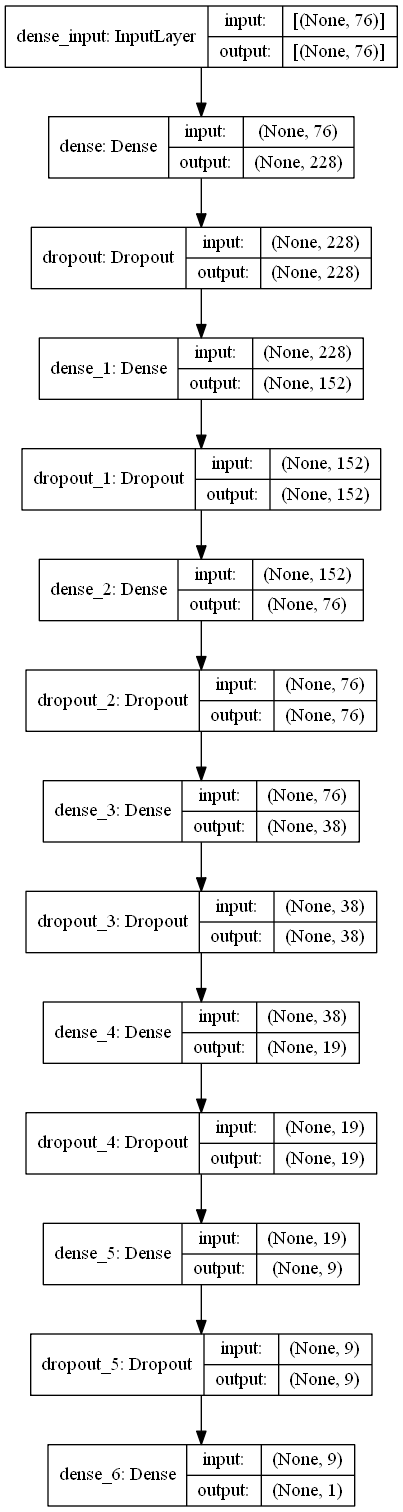
\includegraphics[scale = 0.35]{images/model_plot.png}
\smallbreak
\caption {Figure 1. Custom DNN Architecture diagram}
\smallbreak
\smallbreak
\smallbreak

The DNN had dropout layers between each of the dense layer that dropped 30\% of the nodes, the activation function for all the layers was the Rectified Linear Unit Function (ReLU). The optimizer for the model was Adam with a learning rate of 0.001, with the metric as Mean Squared Error (MSE). L2 Loss kernel regularization was also added to reduce L2 loss (MSE), as that is the evaluation metric of choice for this project.
%%%%%%%%%%%%%%%%
\section{Results}

\subsection{Exploratory Data Analysis}

In order to contextualize the results of the models', some statistics and data-visualizations of the target value and input features from the initial exploratory data analysis that were carried out would help put the performance metrics of the models.
\smallbreak
\smallbreak
\smallbreak
\footnotesize
\begin{tabular}{|l|l|}
\hline
\textit{\textbf{Statistic}} & \textit{\textbf{Value}}                    \\ \hline
Skew                        & 6.096520           \\ \hline
Kurtosis                    & 47.792884          \\ \hline
Count                       & 1844               \\ \hline
Mean                        & 2107441.4446854666 \\ \hline
Standard   deviation        & 2949678.5712087657 \\ \hline
Min                         & 220000.0           \\ \hline
Max                         & 35000000.0         \\ \hline
50th   percentile           & 1425000.0                                  \\ \hline
\end{tabular}
\smallbreak
\centrecaption{TABLE 4. Target value statistics}
\smallbreak
\normalsize

The statistics in Table 4 might not mean much in a vacuum, but will prove to be crucial when determining the performance of different models.

\smallbreak
\smallbreak
\smallbreak
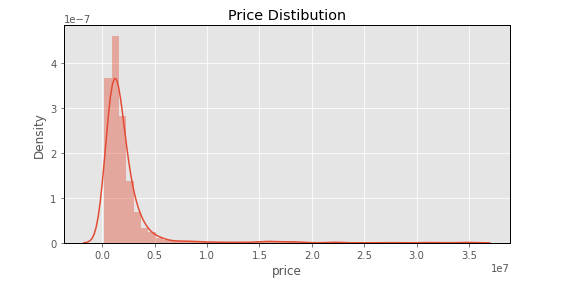
\includegraphics[scale = 0.6]{images/pricefig.png}
\smallbreak
\caption {Figure 2. Price kernel density estimate (KDE)}
\smallbreak
\smallbreak
\smallbreak

Looking at the Kernel Density Estimate (KDE) of the price in Figure 2, it is immediately obvious that the price distribution is extremely right skewed. There are some apartments that cost significantly more than others, and its likely that the prices follow a Pareto process ( a power law distribution where a minority of the inputs account for a majority of the outputs, for example the 80-20 Rule, or Moore's Law). 

Furthermore, Figure 2 helps intuit that Gaussian models like Bayesian Regression would probably not be the best fit for the data set as they rely on normally distributed inputs and outputs to perform optimally.

Further data visualizations helped intuit more things about the nature of the primary data set that isn't immediately obvious looking at Table 4, and thus helped to understand not only how to get the most out of the models but to understand the limitations of the predictions as well. 

\smallbreak
\smallbreak
\smallbreak
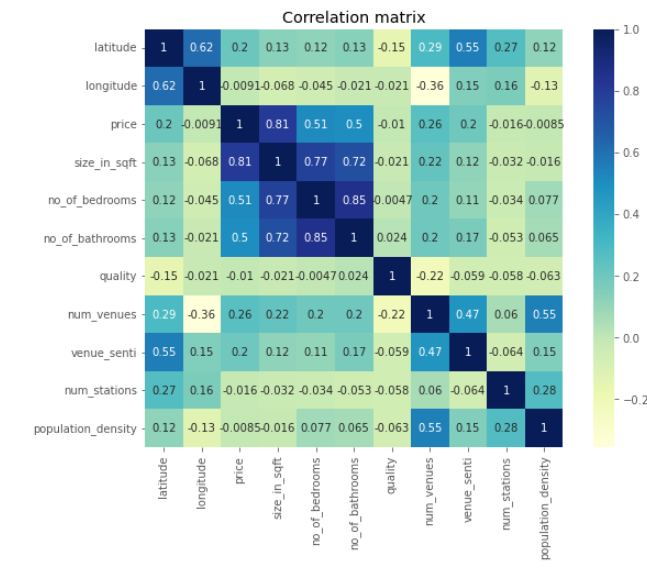
\includegraphics[scale = 0.45]{images/numerical_features_corrmat.png}
\smallbreak
\caption {Figure 3. Correlation matrix of price and numerical features}
\smallbreak
\smallbreak
\smallbreak

Some interesting (wrong) conclusions can be reached if one were to only observe the correlation matrix in Figure 3. For example it price is very strongly correlated with the size of the apartment, which it is, but is far from the most important features (determined by f-score), which will be revealed via carrying out a Principle Component Analysis (PCA) of the features, post training and evaluating the models. This is worth mentioning because premature optimization of the model obtained from insights during the EDA phase can lead model optimization astray. 

\smallbreak
\smallbreak
\smallbreak
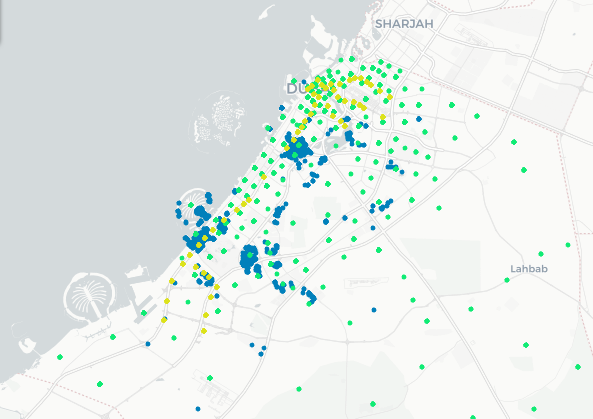
\includegraphics[scale = 0.5]{images/locations_dataviz.png}
\smallbreak
\caption {Figure 4. Apartments (blue), Metro Stations (yellow), Venues (green)}
\smallbreak
\smallbreak
\smallbreak

More on the topic of weaknesses of the data set. Figure 4 is a geospatial scatter-plot of apartments, metro stations and venues, from 3 of the different data sets mentioned in Table 1. It is immediately obvious that a roughly 'decent' amount of the data points will not be utilized effectively by the models. As they are either not in the vicinity of apartments, xor data for the alternate data point doesn't exist in its near vicinity. Moreover, the apartments in the data set are clustered around specific neighborhoods, which preemptively suggests location will probably have an outsized importance in model performance.  


\subsection{XGB}

The XGB model was trained and tested with its default parameters and tuned parameters. As discussed previously in Section 6, The model was tuned using the Grid-Search algorithm. 

And the main metric to look out for is the normalized RMSE as it puts the RMSE value in context. RMSE is the metric of choice as discussed previously in Section 2, RMSE punishes outliers more than MAE, and that is of particular relevance when predicting the price of something. 

\smallbreak
\smallbreak
\smallbreak
\footnotesize
\begin{tabular}{|l|l|l}
\hline
                            & XGB   default (AED) & XGB tuned  \\ \hline
MAE                         & 482732.71           & 586615.38  \\ \hline
RMSE                        & 1491073.48          & 1289409.33 \\ \hline
Normalized   RMSE           & 0.04                & 0.04       \\ \hline
Accuracy (1 – MAPE )*100 & 81.48 \%            & 71.96 \%   \\ \hline
\end{tabular}
\smallbreak
\centrecaption{TABLE 5. Summary, XGB results}
\smallbreak
\smallbreak
\smallbreak
\normalsize

Looking at Table 5 it is evident that when optimizing (to the point of over optimizing) a model for one specific metric, the other metrics suffer. The tuned model does have a lower RMSE than the untuned model, but it comes at the cost of all the other metrics. However The normalized RMSE values for models are quite satisfactory, implying that perhaps tuning the model might be causing it to overfit given the RMSE might not be the best metric for other data sets.

\smallbreak
\smallbreak
\smallbreak
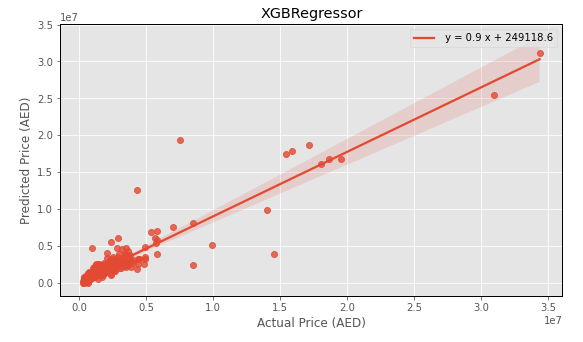
\includegraphics[scale = 0.55]{images/xgb.png}
\caption {Figure 5. Tuned XGB, Actual vs. Predicted plot}
\smallbreak
\smallbreak
\smallbreak

The Actual vs Predicted plot in Figure 5 shows that the model performed relatively well. Even with outlier data, which was not removed intentionally, partly because it is not entirely evident that are the extremely high prices in specific neighborhoods (for example, Palm Jumeirah), actually outlier values with respect to the dataset or representative of the features they carry. Nonetheless The model produced predictions that have a r value of 0.93, a p value of 0.00 and an error of 0.02 (Linear fit). 

\subsection{DNN}

The testing methodology for the DNN was kept exactly the same as the XGB model. Other than a few small changes in the source code (which are irrelevant to the end user), to handle differences in the way the XGB model and the DNN deal with input and output data. The DNN was trained on a Ryzen5 2600, 6 core CPU for 400 epochs.  

\smallbreak
\smallbreak
\smallbreak
\begin{tabular}{|l|
>{\columncolor[HTML]{FFFFFF}}l |}
\hline
                            & DNN        \\ \hline
MAE                         & 619741.69  \\ \hline
RMSE                        & 1267673.33 \\ \hline
Normalized   RMSE           & 0.04       \\ \hline
Accuracy (   1 – MAPE )*100 & 75.86 \%   \\ \hline
\end{tabular}
\smallbreak
\centrecaption{TABLE 6. Summary, DNN results}
\smallbreak

\normalsize

The DNN performed better than the XGB models as evident on Table 6. Which is somewhat surprising because XGB is almost near the ideal model for the data set used in this project. Moreover, the DNN is far from a maximally optimized model (which is not the case with the tuned XGB), not to mention that there is much room for improvement in the architecture. 


\smallbreak
\smallbreak
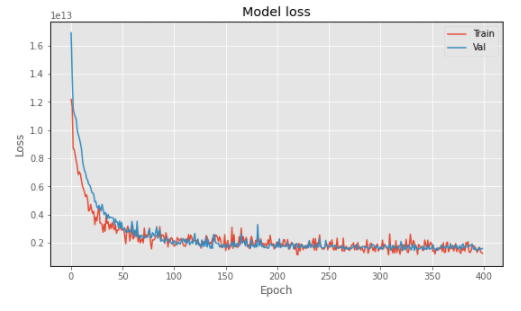
\includegraphics[scale = 0.6]{images/history.png}
\caption {Figure 6. DNN training history}
\smallbreak


However, it is not to say that the architecture is lacklustre, given the performance is better than XGB, and the training history plot in Figure 6 shows loss was very similar across both training and testing datasets, as they converge to their final value. This indidicates the model didn't over/underfit and will generalize well across data sets.  


\smallbreak
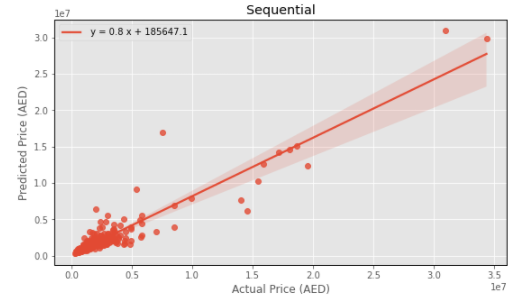
\includegraphics[scale = 0.6]{images/dnn_ap.png}
\caption {Figure 6. DNN training history}
\smallbreak


The Actual vs. Predicted plot of the DNN shows similar predictive performance to the XGB model. With the exact same linear fit metrics; r value of 0.93, p value of 0.00 and error of 0.02. Implying the models performance is very similar. 


\section*{Conclusion}

\smallbreak
\smallbreak
\smallbreak
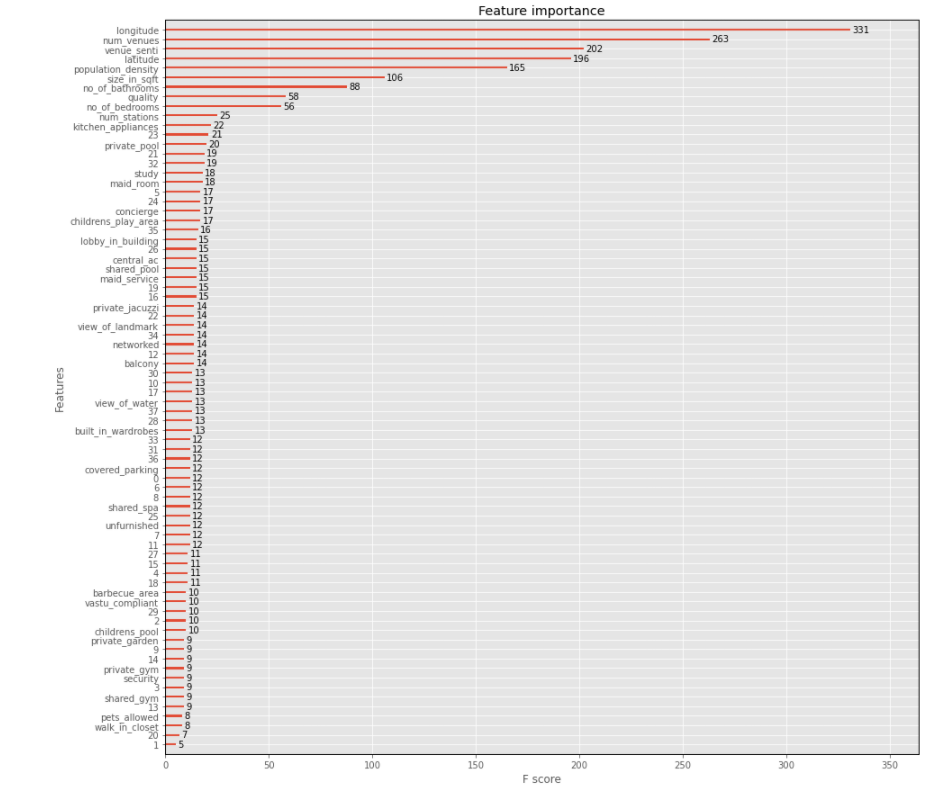
\includegraphics[scale = 0.33]{images/feat_impt.png}
\caption {Figure 8. Feature importance plot from XGB tuned}
\smallbreak
\smallbreak
\smallbreak

Figure 8 is the aforementioned XGB feature importance plot. The reason we are back to the EDA section of the report is to discuss how a exploratory enquiry into a data-science task reveals only half the picture (insights that can be extracted from the data). Figure 8 shows that by far the most out-sized effect on the models' ability to predict was actually the GPS coordinates of the apartment. Which in retrospect seems obvious given that location is an extremely important factor in determining the price of a house. 

As far as improvements are considered, there are three standout and very obvious improvements that would increase the models' predictive ability. The first one being that the sales data in this data set was not time-delineated; Which significantly weakens the real world predictive ability of a model given that prices of most things, especially real-estate vary and fluctuate over time, as a function of time and surrounding events. 

Secondly, A more information dense data set would be desirable. 1800 data points is a fairly small amount of data for Neural Network based models. A more feature rich data set on top of a denser data set would also be desirable given that most of the columns in this data set were Boolean columns.

Finally, a much more sophisticated Neural Network architecture could be conjured up. The DNN used in this paper was a relatively simple DNN that was not tested to the full extent due to time and computational constraints. 



\begin{thebibliography}{1}

\bibitem {Fattah}
Z. Fattah, ’’ Behind the Sizzle of Dubai Home Boom, Key Vulnerability Persists,’’ \emph { Bloomberg News.}, October 7 2021.

\bibitem {zulkifley}
N. H. Zulkifley, S. A. Rahman, N. H. Ubaidullah, and I. Ibrahim, ’’ House Price Prediction using a Machine Learning Model: A Survey of Literature,’’ \emph { International Journal of Modern Education \& Computer Science}, vol. 3, no. 6, pp.46-54, December 2020

\bibitem {chen}
T. Chen, and C. Guestrin, ’’ XGBoost: A Scalable Tree Boosting System,’’ \emph { In Proceedings of the 22nd ACM SIGKDD international conference on knowledge discovery and data mining,}, San Francisco, CA, USA, pp. 785-794, August 13-17 2016.
\bibitem {saikia}
A. Saikia, and S. Paul, ’’ Application of Deep Learning for EEG,’’ \emph { Handbook of Research on Advancements of Artificial Intelligence in Healthcare Engineering.}, p18, 2020.
\bibitem {babu}
S. Babu , ’’ Understanding and Analyzing Deep Neural Networks,’’ \emph { Geek culture.}, April 22 2021.

\bibitem {zaharchuk}
G. Zaharchuk, E. Gong, M. Wintermark, D. Rubin and C.P. Langlotz, ’’ Deep Learning in Neuroradiology,”’’ \emph { American Journal of Neuroradiology.}, February 2018.



\end{thebibliography}

\end{document}